\documentclass{beamer}
\usepackage{color}


\usepackage{listings}
\usepackage[utf8]{inputenc}
\usepackage{default}


\graphicspath{{img/}}

\usepackage{showexpl}

\definecolor{codebg}{HTML}{F3D5F5}

\lstset{language=Python,
breakatwhitespace=false, showspaces=false, showtabs=false, breakatwhitespace=false, breaklines=false, 
backgroundcolor=\color{codebg}}

\lstdefinestyle{highlight}{keywordstyle=\color{blue},
breakatwhitespace=false, showspaces=false, showtabs=false, breakatwhitespace=false, breaklines=false, 
commentstyle=\ttfamily\color{purple}}
\lstdefinestyle{base}{
%   language=Python,
  basicstyle=\ttfamily\color{codebg},
  breakatwhitespace=false, showspaces=false,showstringspaces=false, showtabs=false, breakatwhitespace=false, breaklines=false, 
  keywordstyle=\color{codebg},
  commentstyle=\ttfamily\color{codebg},
  moredelim=**[is][\only<1->{\color{black}\lstset{style=highlight}}]{@}{@},
  moredelim=**[is][\only<1->{\color{black}\lstset{style=highlight}}]{@1}{@},
  moredelim=**[is][\only<2->{\color{black}\lstset{style=highlight}}]{@2}{@},
  moredelim=**[is][\only<3->{\color{black}\lstset{style=highlight}}]{@3}{@},
  moredelim=**[is][\only<4->{\color{black}\lstset{style=highlight}}]{@4}{@},
  moredelim=**[is][\only<5->{\color{black}\lstset{style=highlight}}]{@5}{@},
  moredelim=**[is][\only<6->{\color{black}\lstset{style=highlight}}]{@6}{@},
  moredelim=**[is][\only<7->{\color{black}\lstset{style=highlight}}]{@7}{@},
  moredelim=**[is][\only<8->{\color{black}\lstset{style=highlight}}]{@8}{@},
  moredelim=**[is][\only<9->{\color{black}\lstset{style=highlight}}]{@9}{@}, 
  moredelim=**[is][\only<1>{\color{black}\lstset{style=highlight}}]{~}{~},
  moredelim=**[is][\only<1>{\color{black}\lstset{style=highlight}}]{~1}{~},
  moredelim=**[is][\only<2>{\color{black}\lstset{style=highlight}}]{~2}{~},
  moredelim=**[is][\only<3>{\color{black}\lstset{style=highlight}}]{~3}{~},
  moredelim=**[is][\only<4>{\color{black}\lstset{style=highlight}}]{~4}{~},
  moredelim=**[is][\only<5>{\color{black}\lstset{style=highlight}}]{~5}{~},
  moredelim=**[is][\only<6>{\color{black}\lstset{style=highlight}}]{~6}{~},
  moredelim=**[is][\only<7>{\color{black}\lstset{style=highlight}}]{~7}{~},
  moredelim=**[is][\only<8>{\color{black}\lstset{style=highlight}}]{~8}{~},
  moredelim=**[is][\only<9>{\color{black}\lstset{style=highlight}}]{~9}{~}
%   texcl=true,escapebegin=\hskip-6cm\color{red}
}

% \lstset{style=base}

\begin{document}


\begin{frame}
% % \frametitle{What is programming?}
% \framesubtitle{It is like use using any other language!}
% 
% ``Getting an education was a bit like a communicable sexual disease. It made you unsuitable for a lot of jobs and then you had the urge to pass it on.''
% \\ \
\centering\Huge Welcome to the computational cognitive modelling workshop! 
\vfill \huge
\centering\textbf{Part 1: Basic programming} \normalsize

\vfill
% \textit{Olivia Guest \hfill  Chris Brand \\  \ Nick Sexton \hfill Nicole Cruz De Echeverria Loebell } 
% -- \textit{Terry Pratchett}
\end{frame}

\begin{frame}
% % \frametitle{What is programming?}
% \framesubtitle{It is like use using any other language!}
% 
% ``Getting an education was a bit like a communicable sexual disease. It made you unsuitable for a lot of jobs and then you had the urge to pass it on.''
% \\ \
\vfill \Huge
\centering Part 1: \textbf{Basic programming} \large

\vfill
\textit{
Olivia Guest \hfill  Chris Brand 
\vspace{0.5cm} \\ \ 
Nick Sexton \hfill Nicole Cruz De Echeverria Loebell } 
% -- \textit{Terry Pratchett}
\end{frame}


\begin{frame}
\frametitle{What is programming?}
\centering \huge 

\begin{figure}

\includegraphics[scale=0.28]{hack.jpg}
\end{figure}
% \framesubtitle{It is like use using any other language!}
% \large
% \begin{itemize}
%  \item Programming = telling a computer what to do \\ \
% % \begin{itemize}
% %   \item The good thing about computers is they do exactly what you tell them, no more and no less.
% %  \item This might be why programmers are bossy and get upset when things in the real world do not go their way!
% % \end{itemize}
% 
% % \item Like speaking any other language \\ \
% 
% \item \textbf{Anybody can program} \\ \
% 
% \item But not everybody is Maya Angelou or Jane Austen! \\ \
% 
% \item But who cares? We can still communicate!

%  \item Some people think programming is an art, a craft, or a type of engineering.
% 
% \begin{itemize}
%   \item We think it is all of the above. 
% \end{itemize}

%  \item Programming and programmers are what bring you things like video games, presentations, and Word!
% \end{itemize}
\end{frame}

\begin{frame}
\frametitle{It is like use using any other language!}
% \centering
%  \huge It is like use using any other language!

\large
\begin{itemize}
 \item Programming = telling a computer what to do \\ \
% \begin{itemize}
%   \item The good thing about computers is they do exactly what you tell them, no more and no less.
%  \item This might be why programmers are bossy and get upset when things in the real world do not go their way!
% \end{itemize}

% \item Like speaking any other language \\ \
\item You write the recipe, the computer follows it \\ \

 \item Programming is an art, a craft, or a type of engineering.
% 
% \begin{itemize}
%    \item We think it is all of the above. 
% \end{itemize}

%  \item Programming and programmers are what bring you things like video games, presentations, and Word!
\end{itemize}
\end{frame}

\begin{frame}
\frametitle{Who is a programmer?}
% \framesubtitle{Why speak or write?}
\large




\begin{figure}
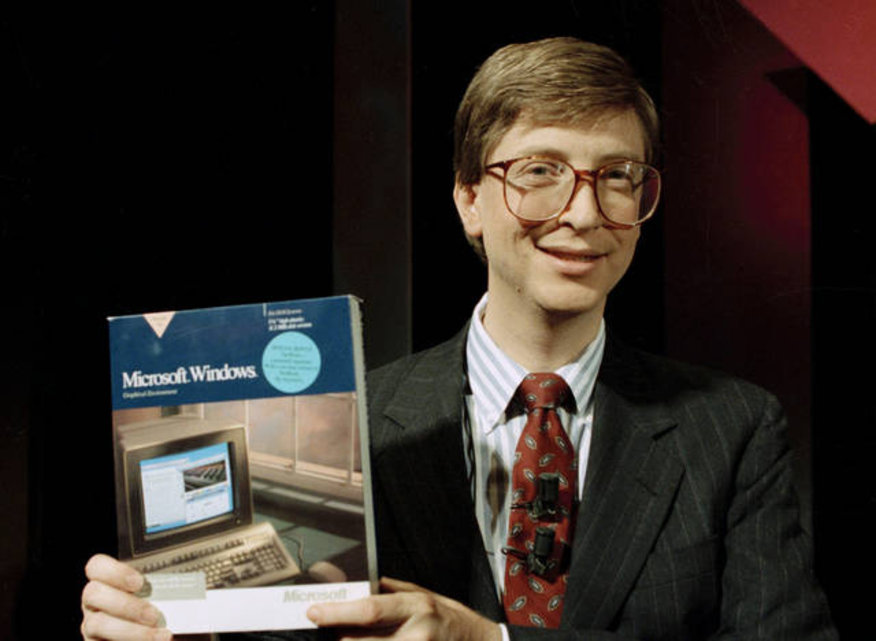
\includegraphics[scale=0.9]{gates.jpg}
\end{figure}
% \begin{itemize}
%  \item Communicate ideas unambiguously \\ \
% 
% \item Allow your ideas to ``live'' on their own \\ \
% 
% \item It is actually fun and definitely addictive \\ \
% 
% \item All the cool kids are doing it
% 
% \end{itemize}

%More content goes here
\end{frame}
\begin{frame}
\frametitle{Who is a programmer?}
\framesubtitle{Ada Lovelace, Grace Hopper, Amanda Spann, etc.}
\large

\begin{figure}
% 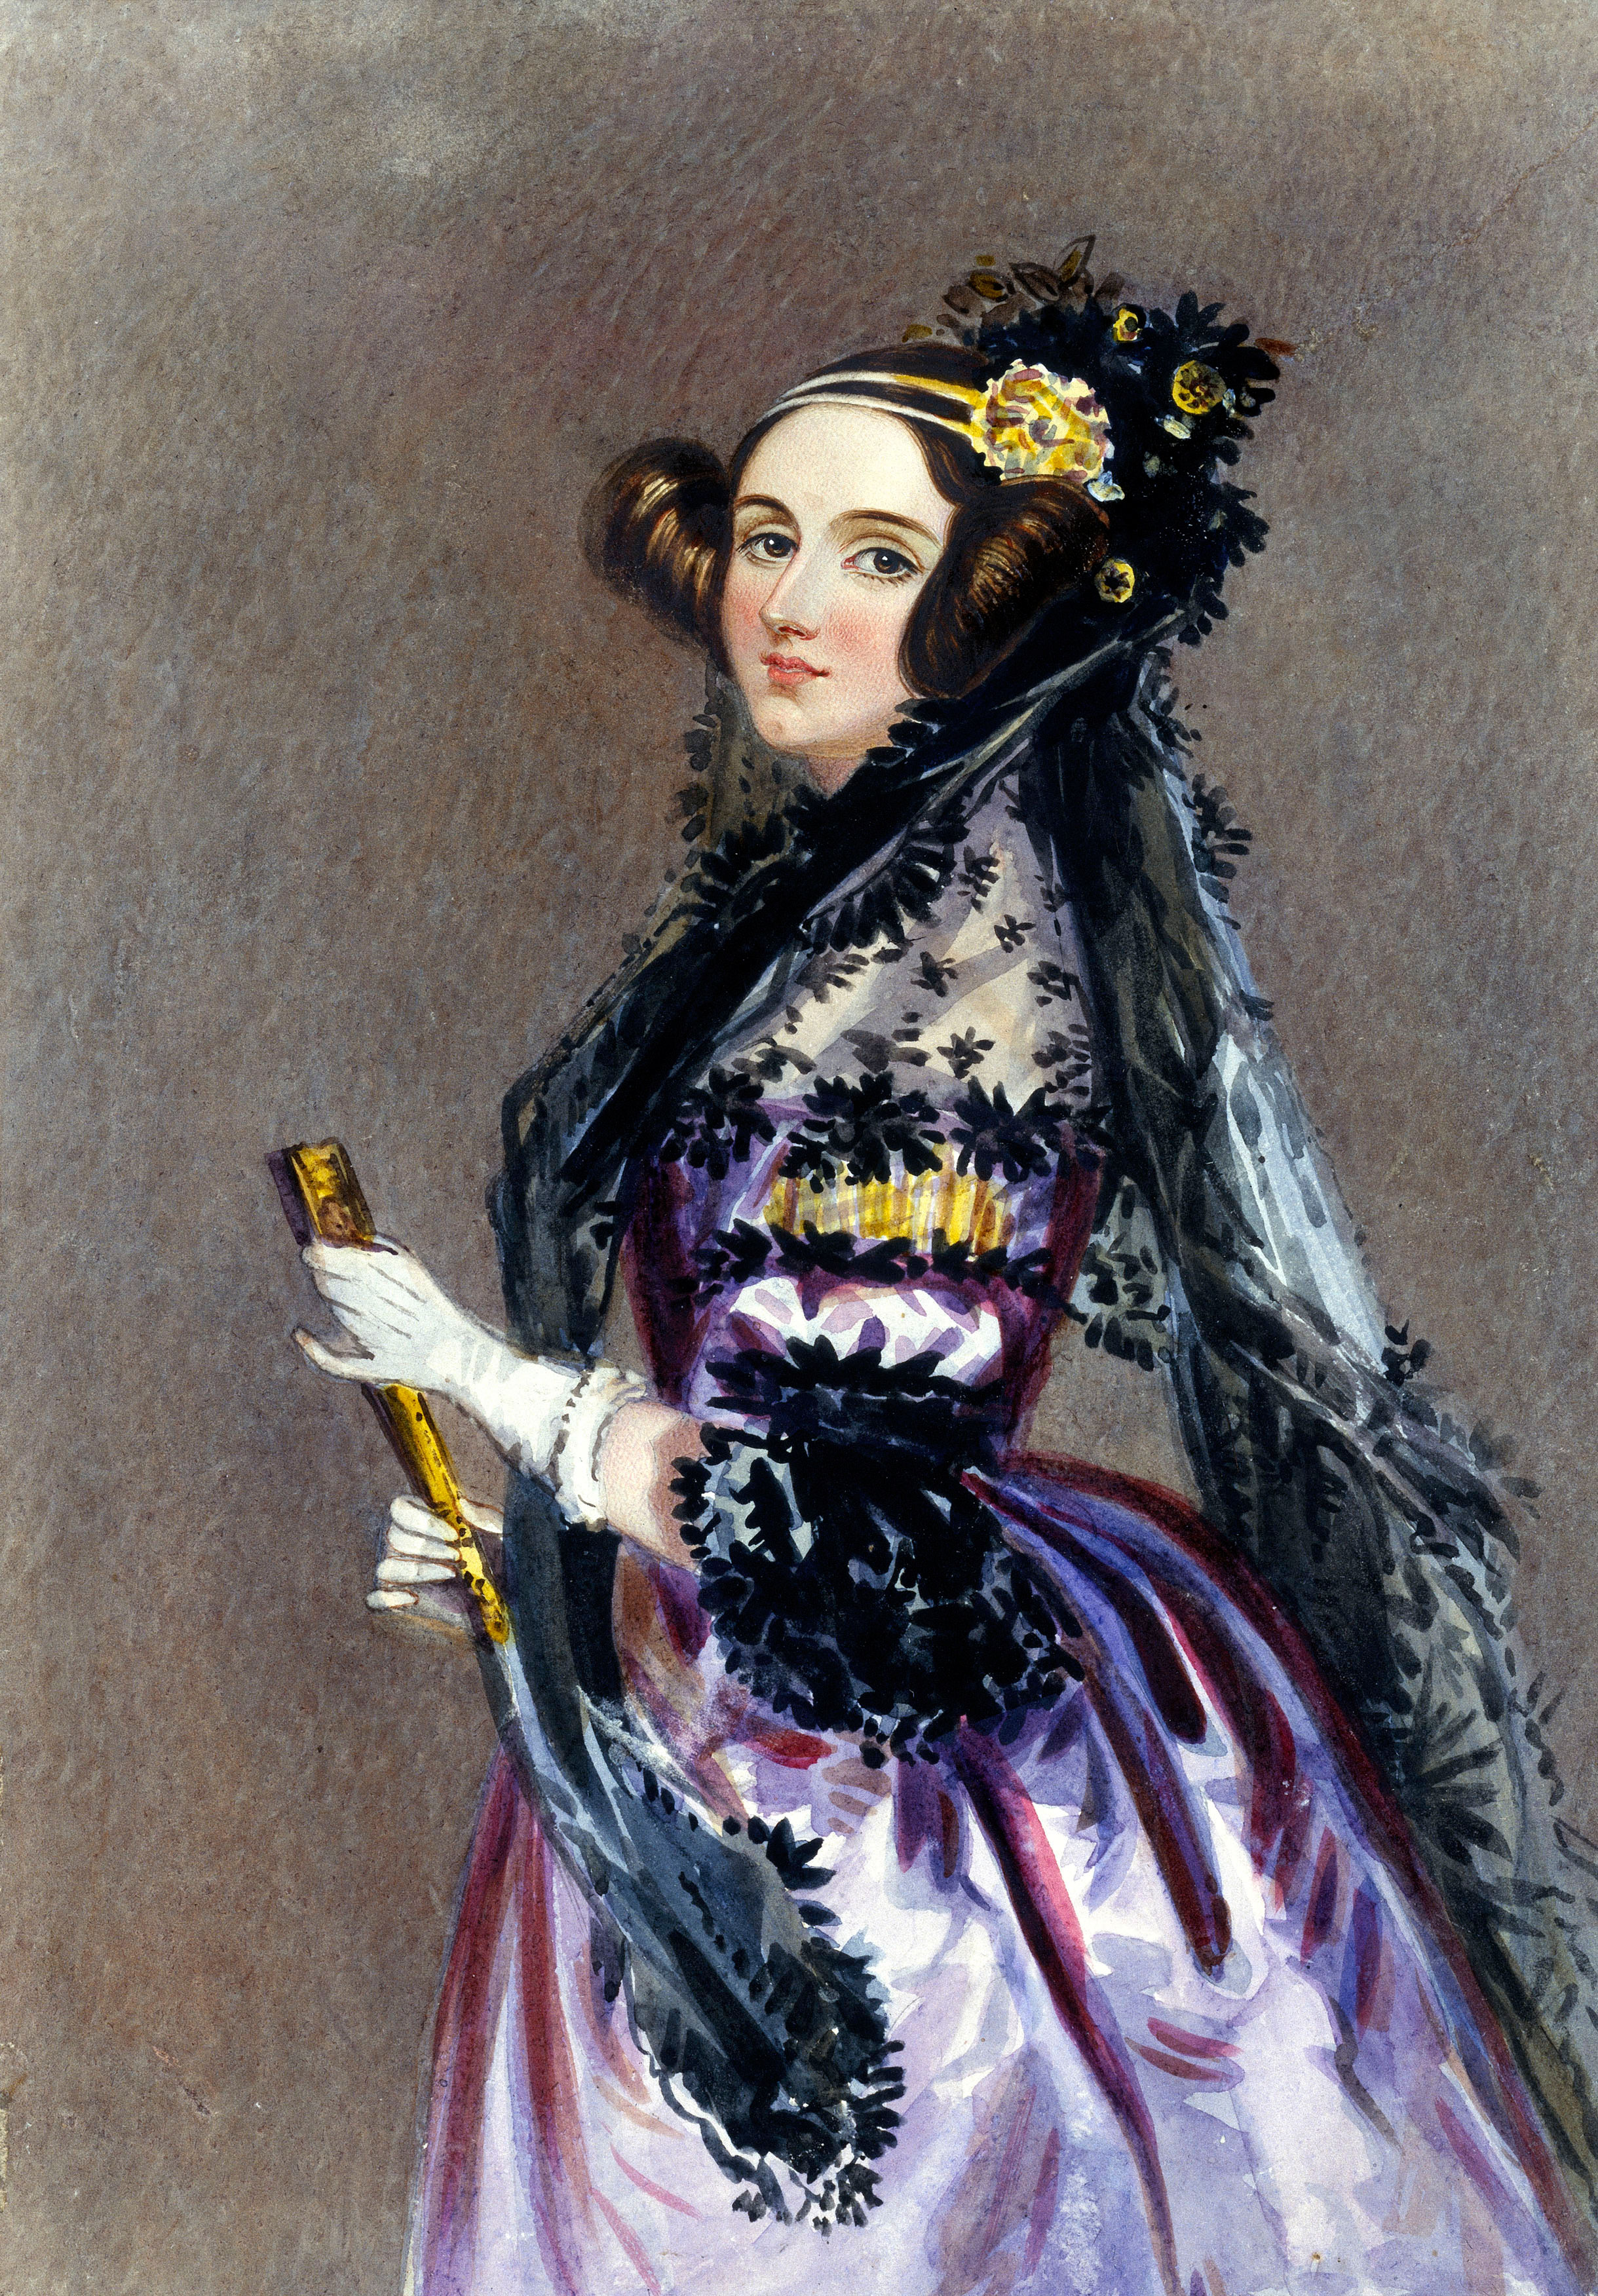
\includegraphics[height=6cm, clip = true, trim = 15cm 5cm 5cm 10cm]{ada.jpg}
% 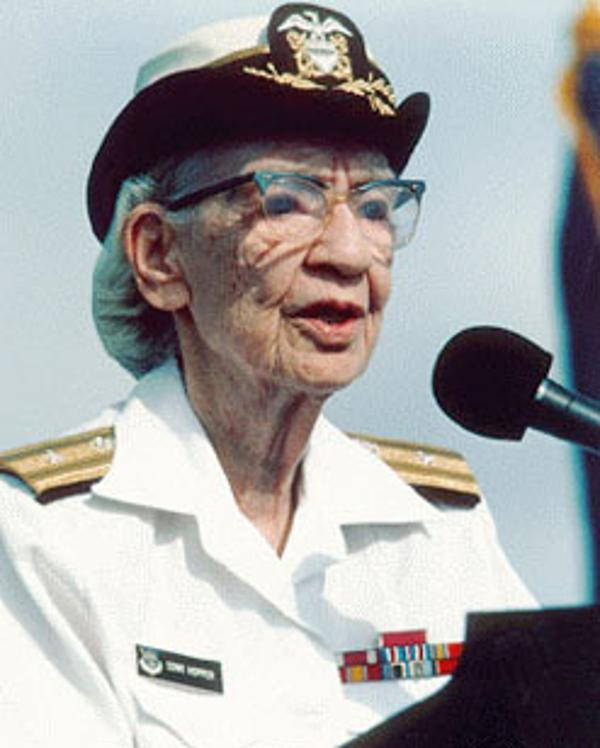
\includegraphics[height=6cm, clip = true, trim = 1cm 5cm 5cm 0cm]{grace.jpg}
% 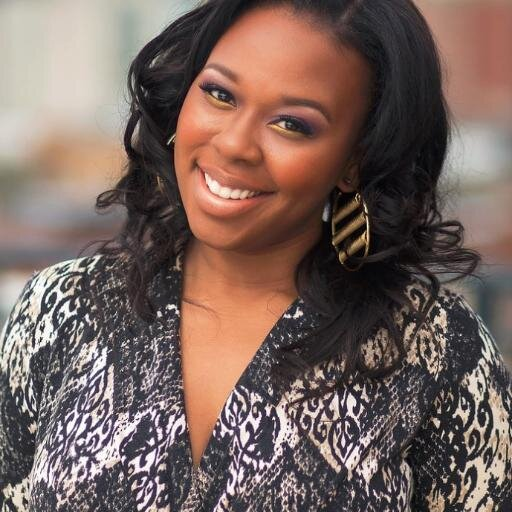
\includegraphics[height=6cm, clip = true, trim = 5cm 1cm 3cm 0cm]{spann.jpeg}
 

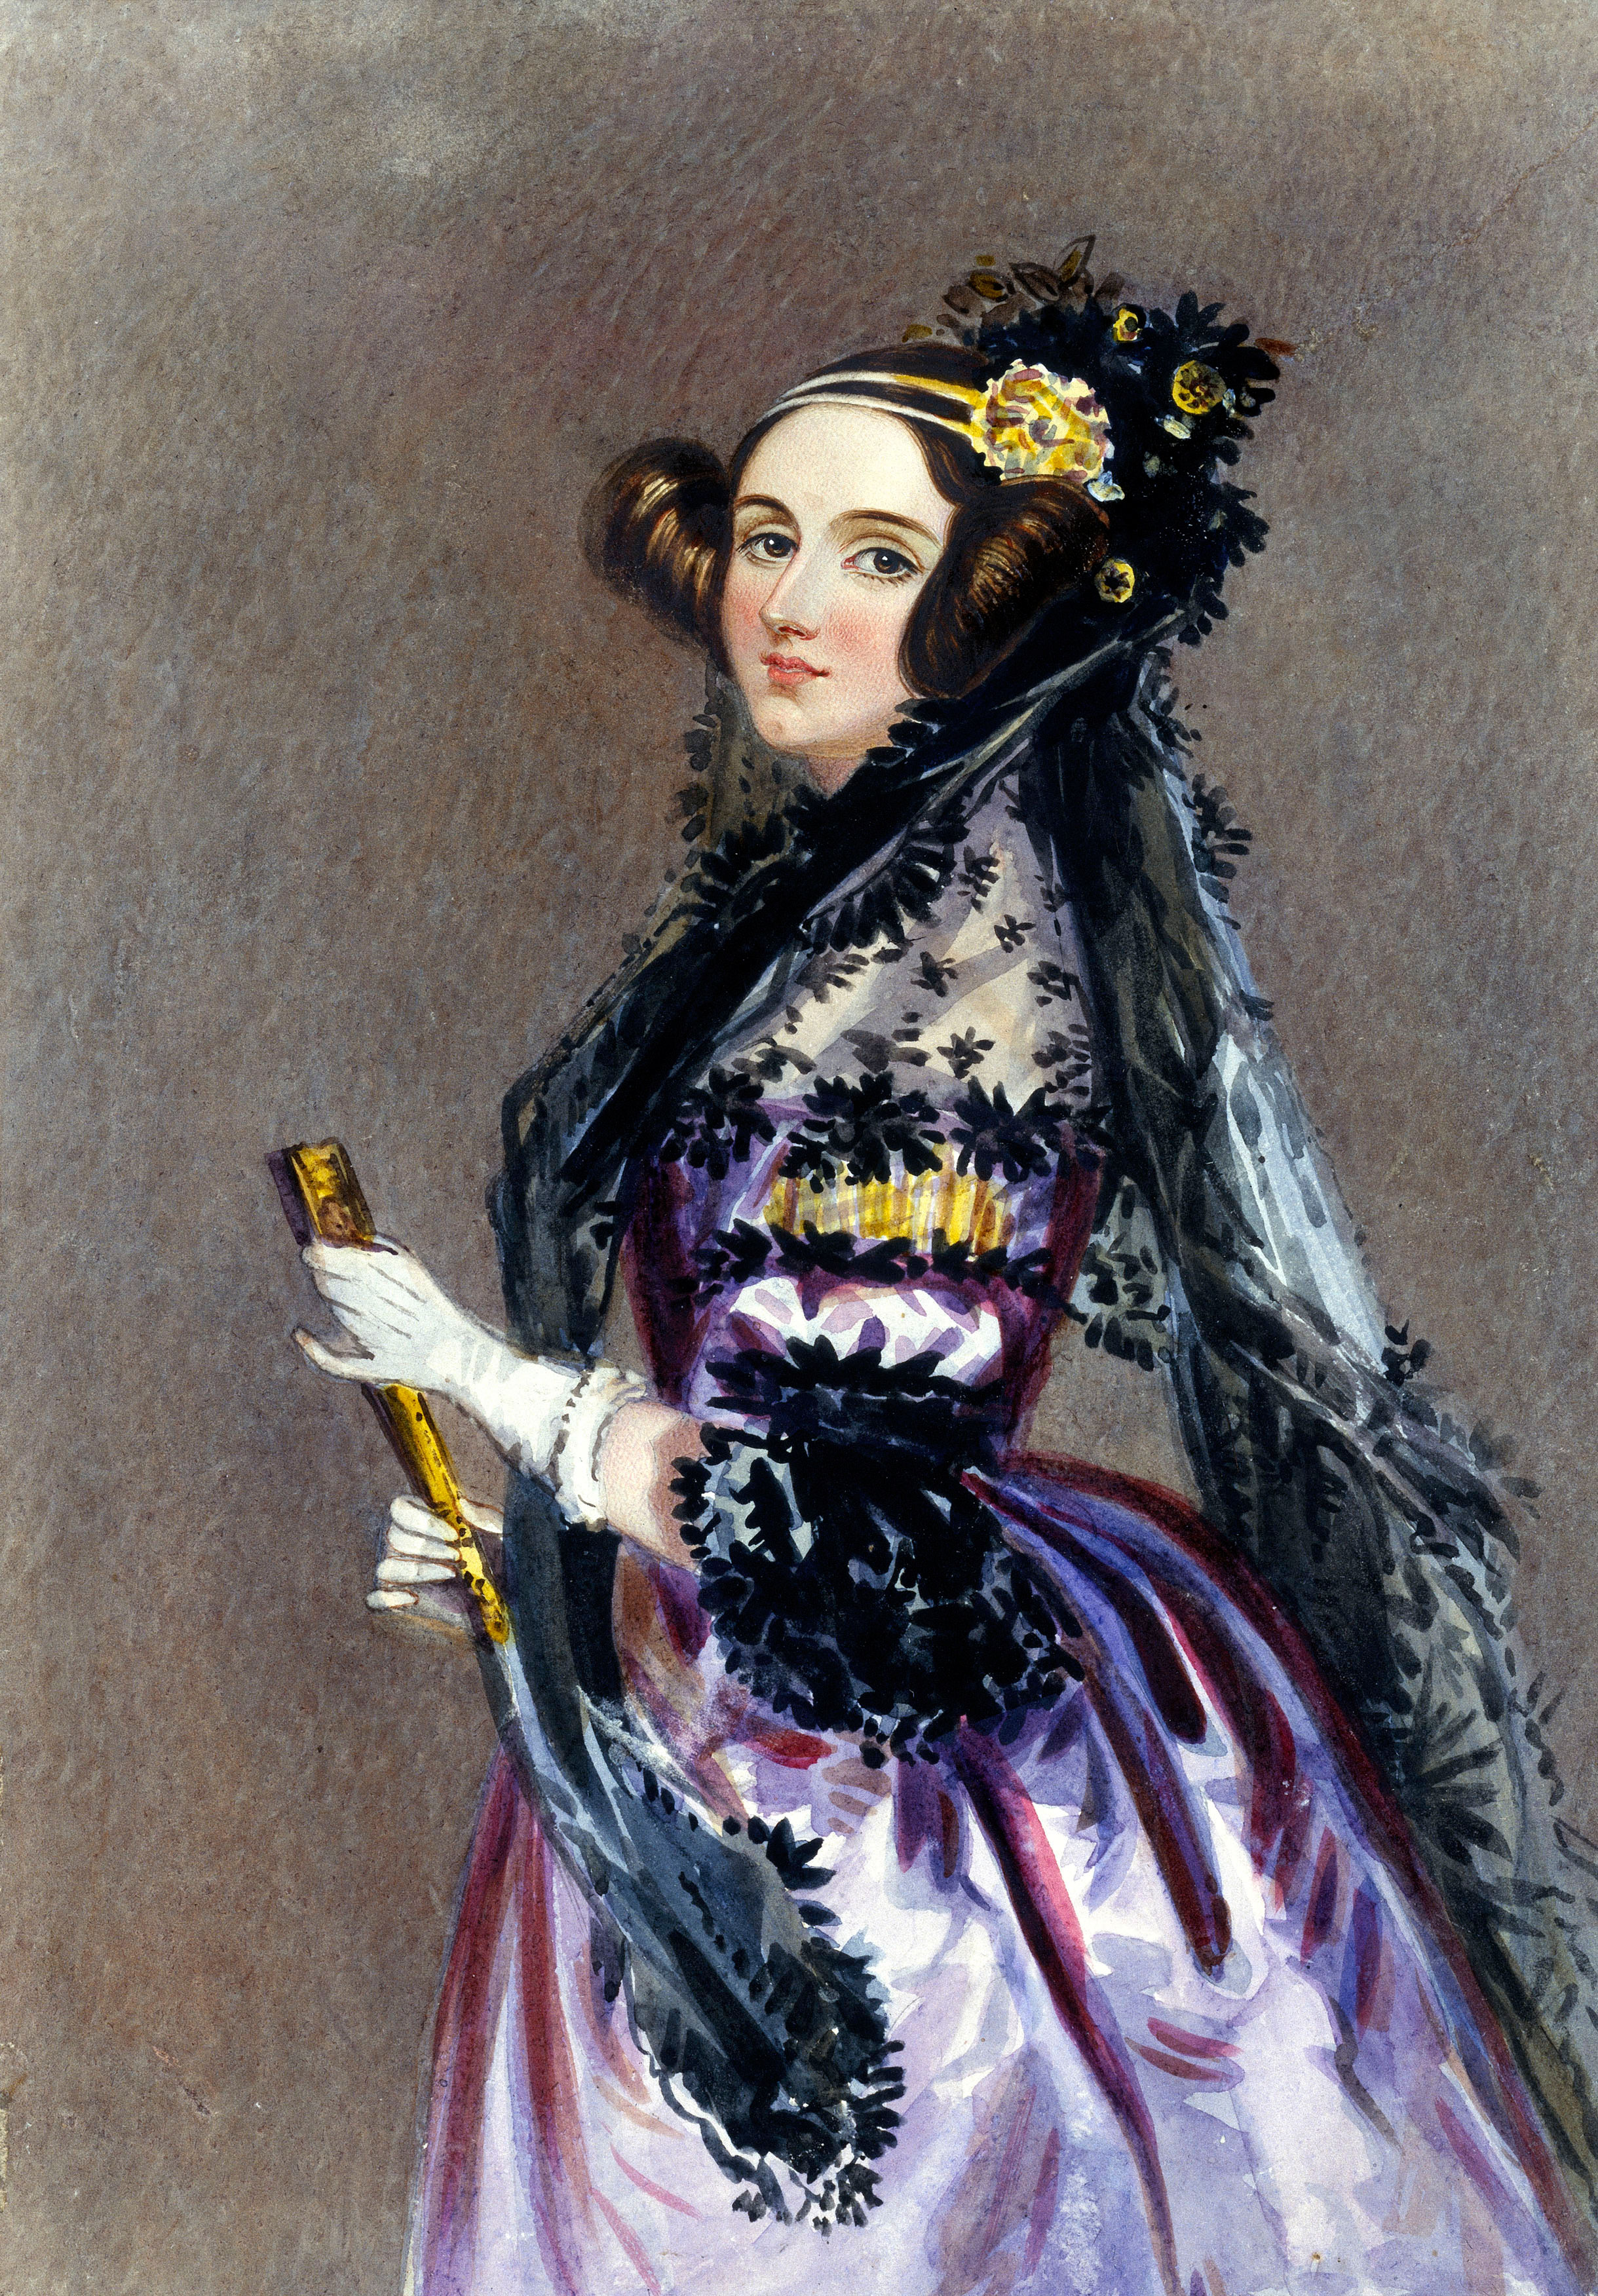
\includegraphics[width=0.333\linewidth, clip = true, trim = 15cm 5cm 5cm 10cm]{ada.jpg}
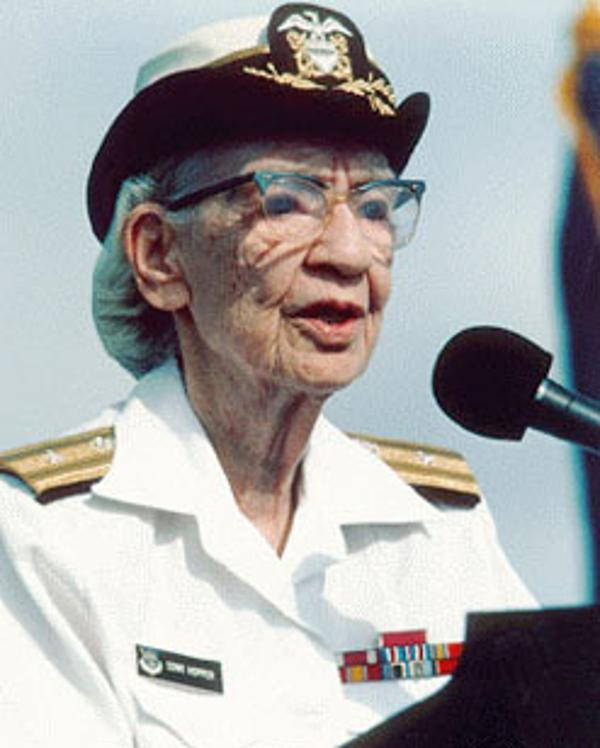
\includegraphics[width=0.333\linewidth, clip = true, trim = 1cm 5cm 5cm 0cm]{grace.jpg}
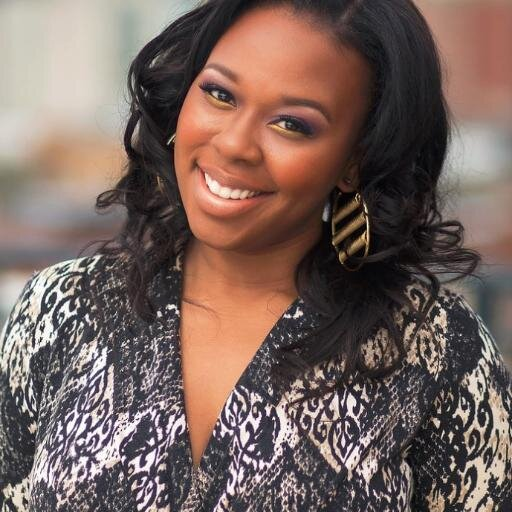
\includegraphics[width=0.333\linewidth, clip = true, trim = 5cm 1cm 3cm 0cm]{spann.jpeg}

\end{figure}

% \begin{itemize}
%  \item Communicate ideas unambiguously \\ \
% 
% \item Allow your ideas to ``live'' on their own \\ \
% 
% \item It is actually fun and definitely addictive \\ \
% 
% \item All the cool kids are doing it
% 
% \end{itemize}

%More content goes here
\end{frame}
\begin{frame}
\frametitle{Who is a programmer?}
\framesubtitle{Children!}
\large

\begin{figure}
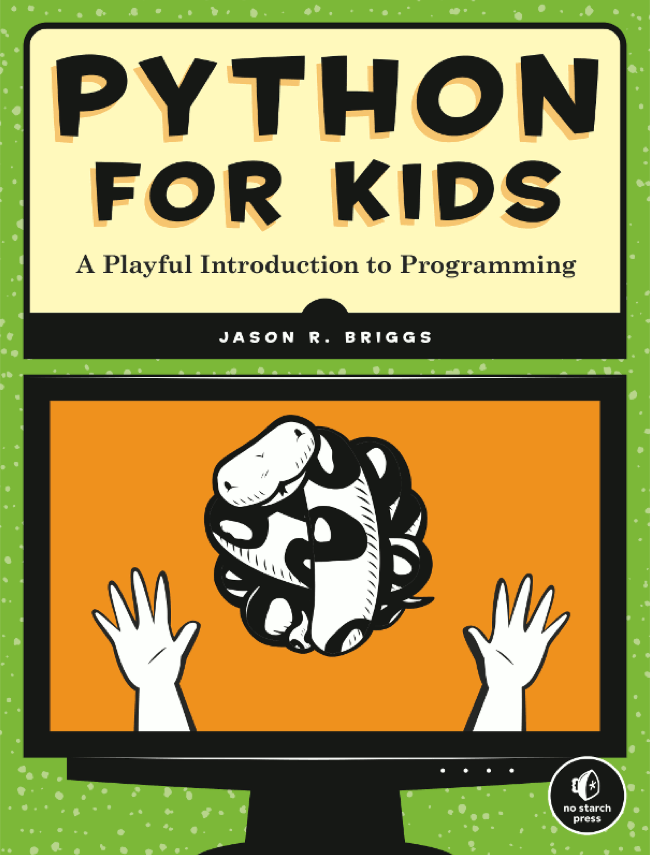
\includegraphics[width=0.4\linewidth]{kids.png}
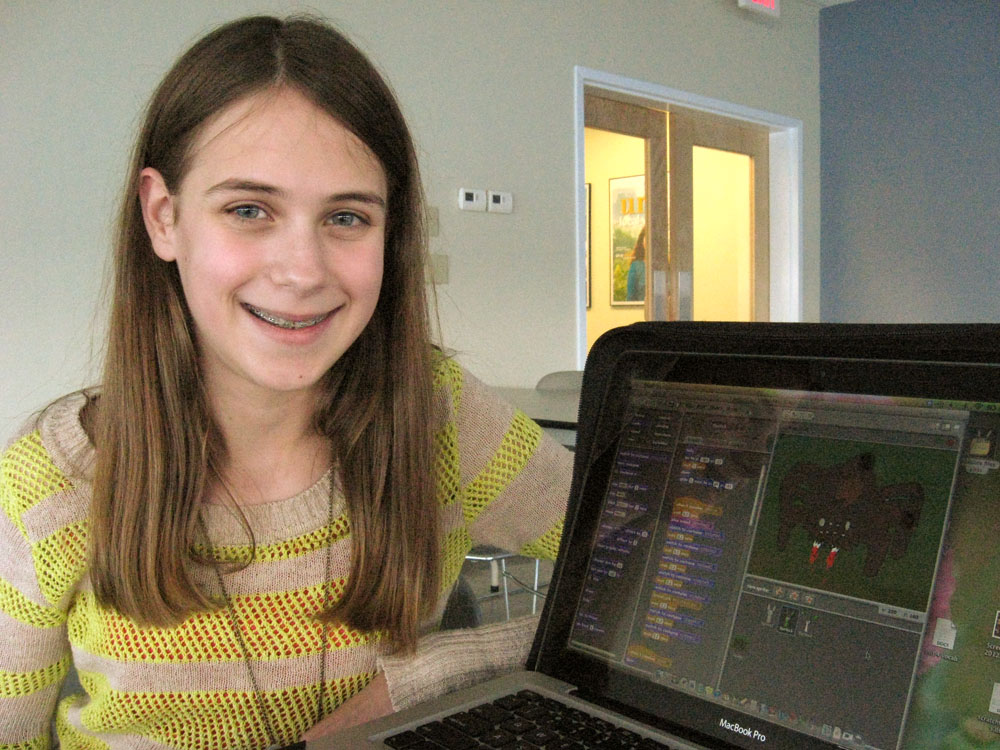
\includegraphics[width=0.6\linewidth]{1226_maddy-petrovich-computer.jpg}
% \caption{Maddy Petrovich, 14, of Wellesley, Mass. first started learning how to use the programming language Scratch when she was 10 years old.}
\end{figure} \small
Maddy Petrovich, 14, of Wellesley, Mass. first started learning how to use the programming language Scratch when she was 10 years old.
\tiny http://hereandnow.wbur.org/2012/12/26/computer-programming-kids

\end{frame}

\begin{frame}
\frametitle{Who is a programmer?}
\framesubtitle{You! Seriously}
\begin{itemize}

\item \textbf{Anybody can program} \\ \

\item But not everybody is Maya Angelou or Jane Austen! \\ \

\item But who cares? We can still communicate! We can still code!
\end{itemize}

\end{frame}


\begin{frame}
\frametitle{Why program?}
\framesubtitle{Why speak or write?}
\large

\begin{itemize}
 \item Communicate ideas unambiguously \\ \

\item Allow your ideas to ``live'' on their own \\ \

\item It is actually fun and definitely addictive \\ \

\item Save time by automating repetitive tasks \\ \

\item All the cool kids are doing it

\end{itemize}

%More content goes here
\end{frame}

\begin{frame}
\frametitle{What is Python?}
\framesubtitle{Will it eat my mouse?}
\begin{figure}

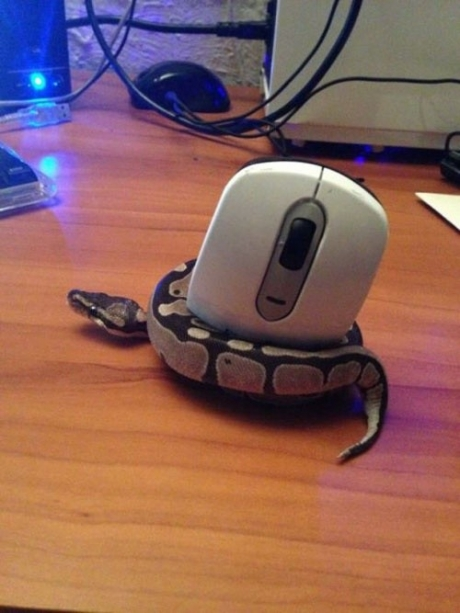
\includegraphics[scale=0.5, clip=true, trim = 0 100px 0 100px]{tumblr_mtrlv0cawn1sjczzeo1_500.jpg}
\end{figure}
\large
\end{frame}

\begin{frame}
\frametitle{What is Python?}
\framesubtitle{Not John Cleese, but closer...}
\begin{figure}

\includegraphics[scale=0.6]{john_cleese1.jpg}
\end{figure}
\large
\end{frame}

\begin{frame}
\frametitle{What is Python?}
\framesubtitle{Not a snake}
\begin{figure}

\includegraphics[scale=0.5]{python_logo.pdf}
\end{figure}
\large

\begin{itemize}

\item Named after Monty Python \\ \

 \item A programming language \\ \
 \item Not scary \\ \
 \item Cool \\ \

\end{itemize}
\end{frame}

\begin{frame}
\frametitle{Who created Python?}
\framesubtitle{A Dutch human}
\begin{figure}

\includegraphics[scale=0.45]{df20000406.jpg}
\end{figure}

% \begin{itemize}
%  \item Guido van Rossum
% \end{itemize}
\end{frame}

\begin{frame}
\frametitle{Who created Python?}
\framesubtitle{Guido van Rossum}
\centering aka Benevolent Dictator For Life

\begin{figure}
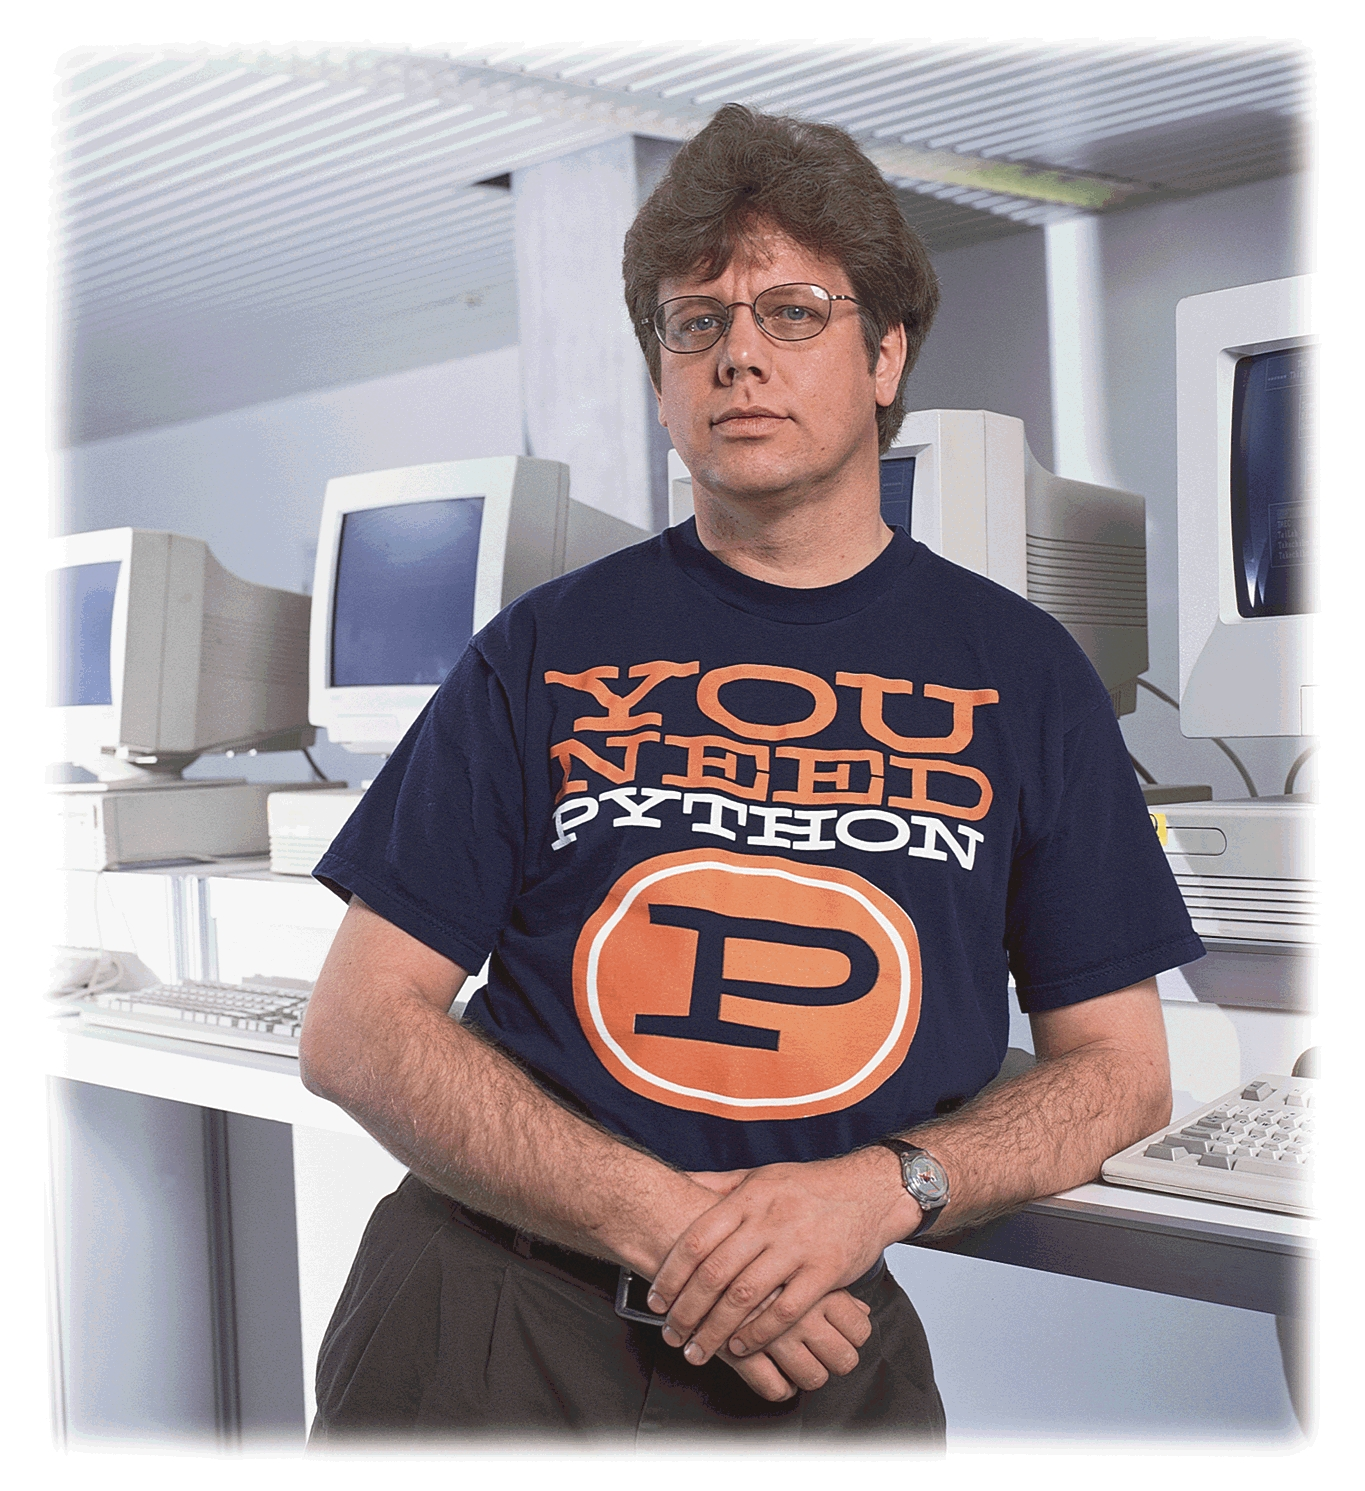
\includegraphics[scale=0.12]{guido.jpg}
\end{figure}
\end{frame}

\begin{frame}
\frametitle{Why use Python?}
\framesubtitle{It was created for you}
\large

\begin{itemize}
% an easy and intuitive language just as powerful as major competitors
% open source, so anyone can contribute to its development
% code that is as understandable as plain English
% suitability for everyday tasks, allowing for short development times

 \item Easy and intuitive \\ \
 \item  Open source and free \\ \

 \item Close to plain English \\ \
 \item Lots of help online \\ \

\item Even geeks like it

\end{itemize}
%More content goes here
\end{frame}


\begin{frame}
\frametitle{Time to get serious!}
\framesubtitle{Open up Python}
\vspace{-1cm}
\begin{figure}
 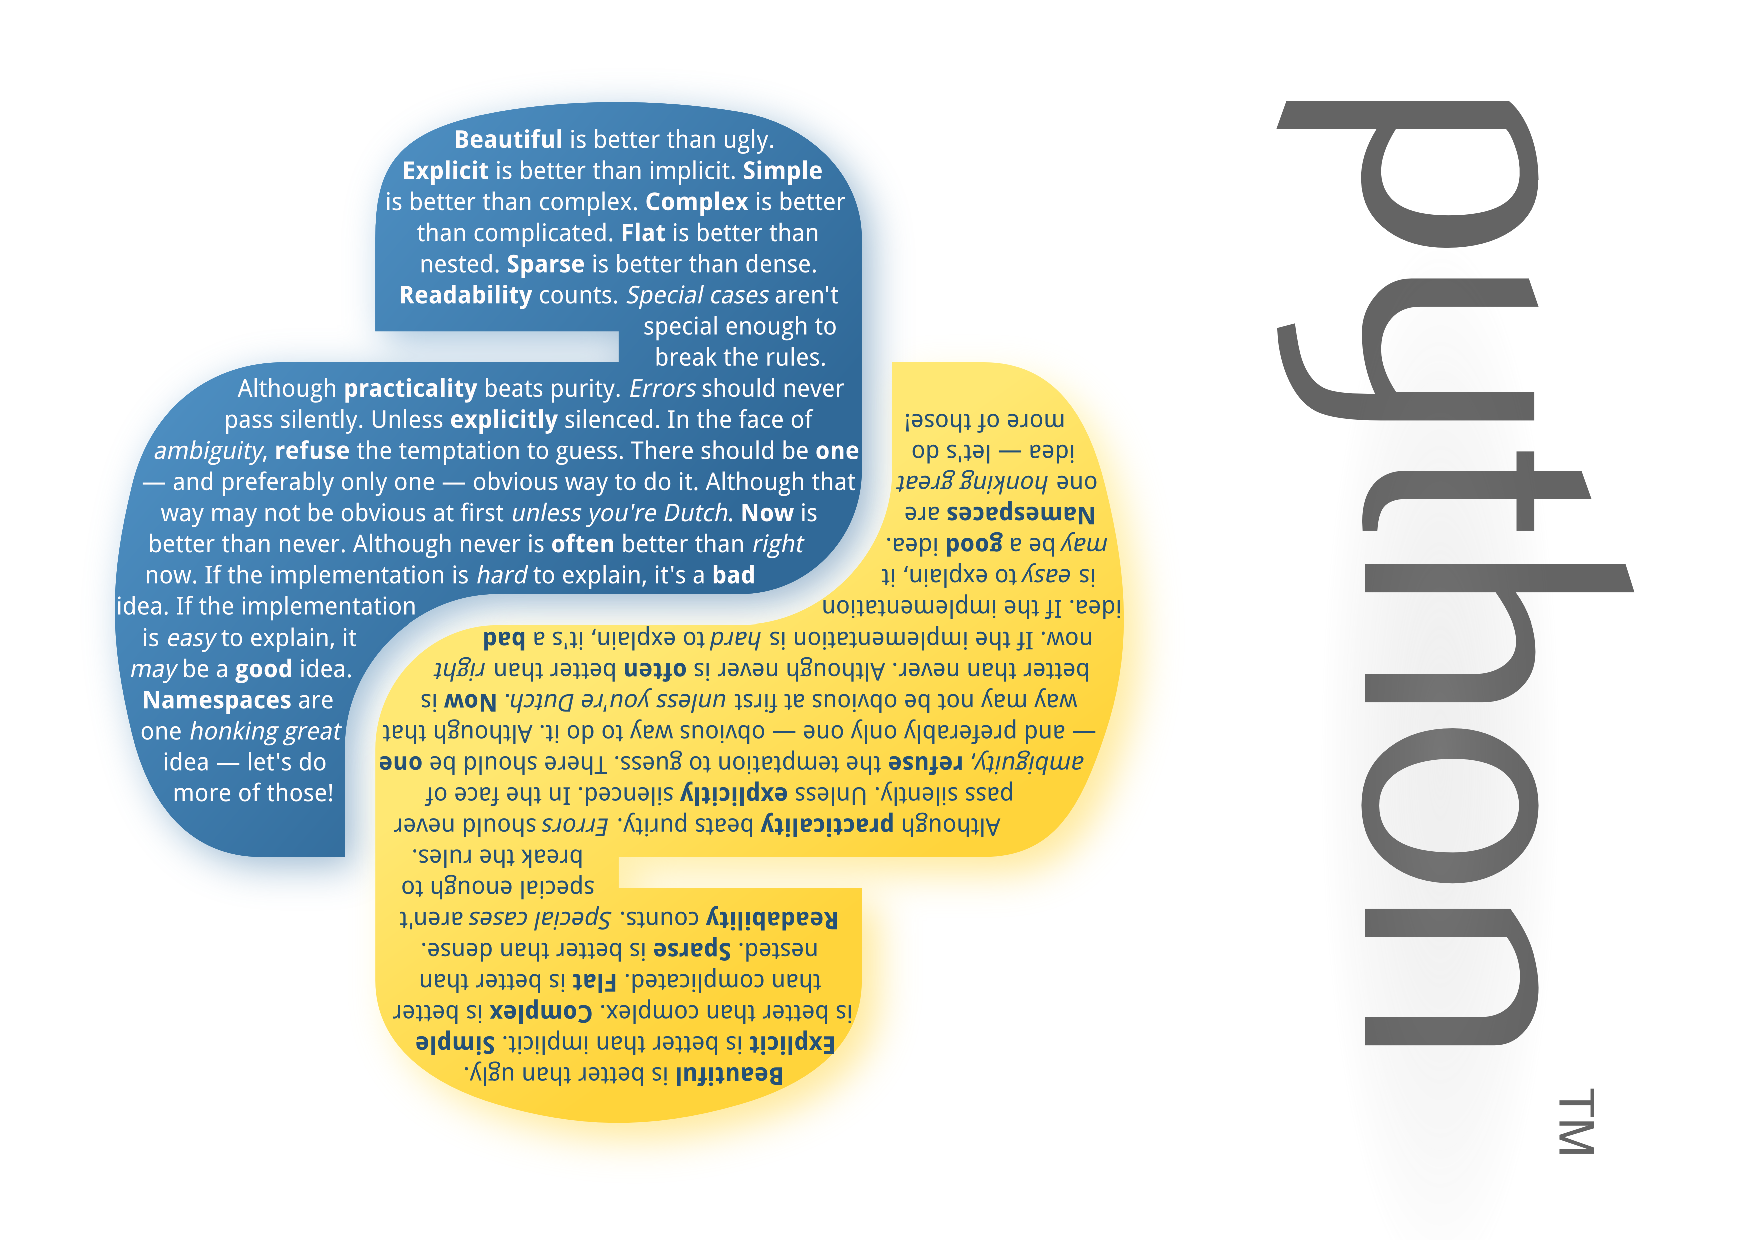
\includegraphics[scale=0.45, clip = true, trim = 0mm  0mm 10cm 0mm]{zen-of-python-poster.pdf}\end{figure}
\end{frame}



\begin{frame}[fragile]
\frametitle{Assignment}
\framesubtitle{Put a value into a variable}
\large
  \begin{columns}[T]
    \begin{column}{.5\textwidth} 
\ \\ 

\ \\ 
\ \\ 

\ \\ 

\begin{itemize}



 \item Does \emph{not} mean equals!\\ \
 \item  Make the variable have the value \\ \

 \item Read as ``assign'', ``make'', or ``equals'' \\ \


\end{itemize}
     \end{column}
     
         \begin{column}{.5\textwidth} 
         Python shell: \\ \
\begin{lstlisting}[style=base]
@2>>> i = 5@
@2>>> print i@
@35@
@4>>> i + 2@
@57@
@6>>> i = i + 1@
@6>>> print i@
@76@
@8>>> i += 0.8@
@97.8
\end{lstlisting}

    \end{column}
    \end{columns}

%More content goes here
\end{frame}


\begin{frame}[fragile]
\frametitle{Basic maths}
\framesubtitle{Arithmetic is fun when you don't have to do it manually!}
\large
  \begin{columns}[T]
    \begin{column}{.5\textwidth} 
\ \\ 

\ \\ 

\ \\ 


\begin{itemize}



 \item Use Python as a calculator\\ \
 \item  Assign results into variables \\ \

 \item All your favourites like plus, minus, times, divided by, etc. \\ \


\end{itemize}
     \end{column}
     
         \begin{column}{.5\textwidth} 
         Python shell: \\ \
\begin{lstlisting}[style=base]
@1>>> (41 + 45.87) / 2@
@243.435@
@3>>> 5**2@
@425@
@5>>> a = 8@
@5>>> b = a / 2@
@5>>> c = b**2@
@6>>> print a, b, c@
@78 4 6@
\end{lstlisting}

    \end{column}
    \end{columns}

%More content goes here
\end{frame}

\begin{frame}[fragile]
\frametitle{Truth values}
\framesubtitle{Perfectly logical}
\large
  \begin{columns}[T]
    \begin{column}{.5\textwidth} 
\ \\ 

\ \\ 


\ \\ 


\begin{itemize}


\item $==$  equality \\ \
\item $!=$ inequality \\ \
 \item$ >=,~ >,~ <=,~ <$\\ \
 \item and, or, not \\ \

%  \item If not sure, ask Python!


\end{itemize}
     \end{column}
     
         \begin{column}{.5\textwidth} 
         Python shell: \\ \
\begin{lstlisting}[style=base]
@1>>> True and False@
@1False@
@2>>> True or False@
@3True@
@4>>> not False@
@5True@
@6>>> 100 == True@
@7False@
@8>>> a != b@
@9True@
\end{lstlisting}

    \end{column}
    \end{columns}

%More content goes here
\end{frame}
%


\begin{frame}
\frametitle{Time to get SUPER serious!}
\framesubtitle{Open a text editor}
\vspace{-1cm}
\begin{figure}
 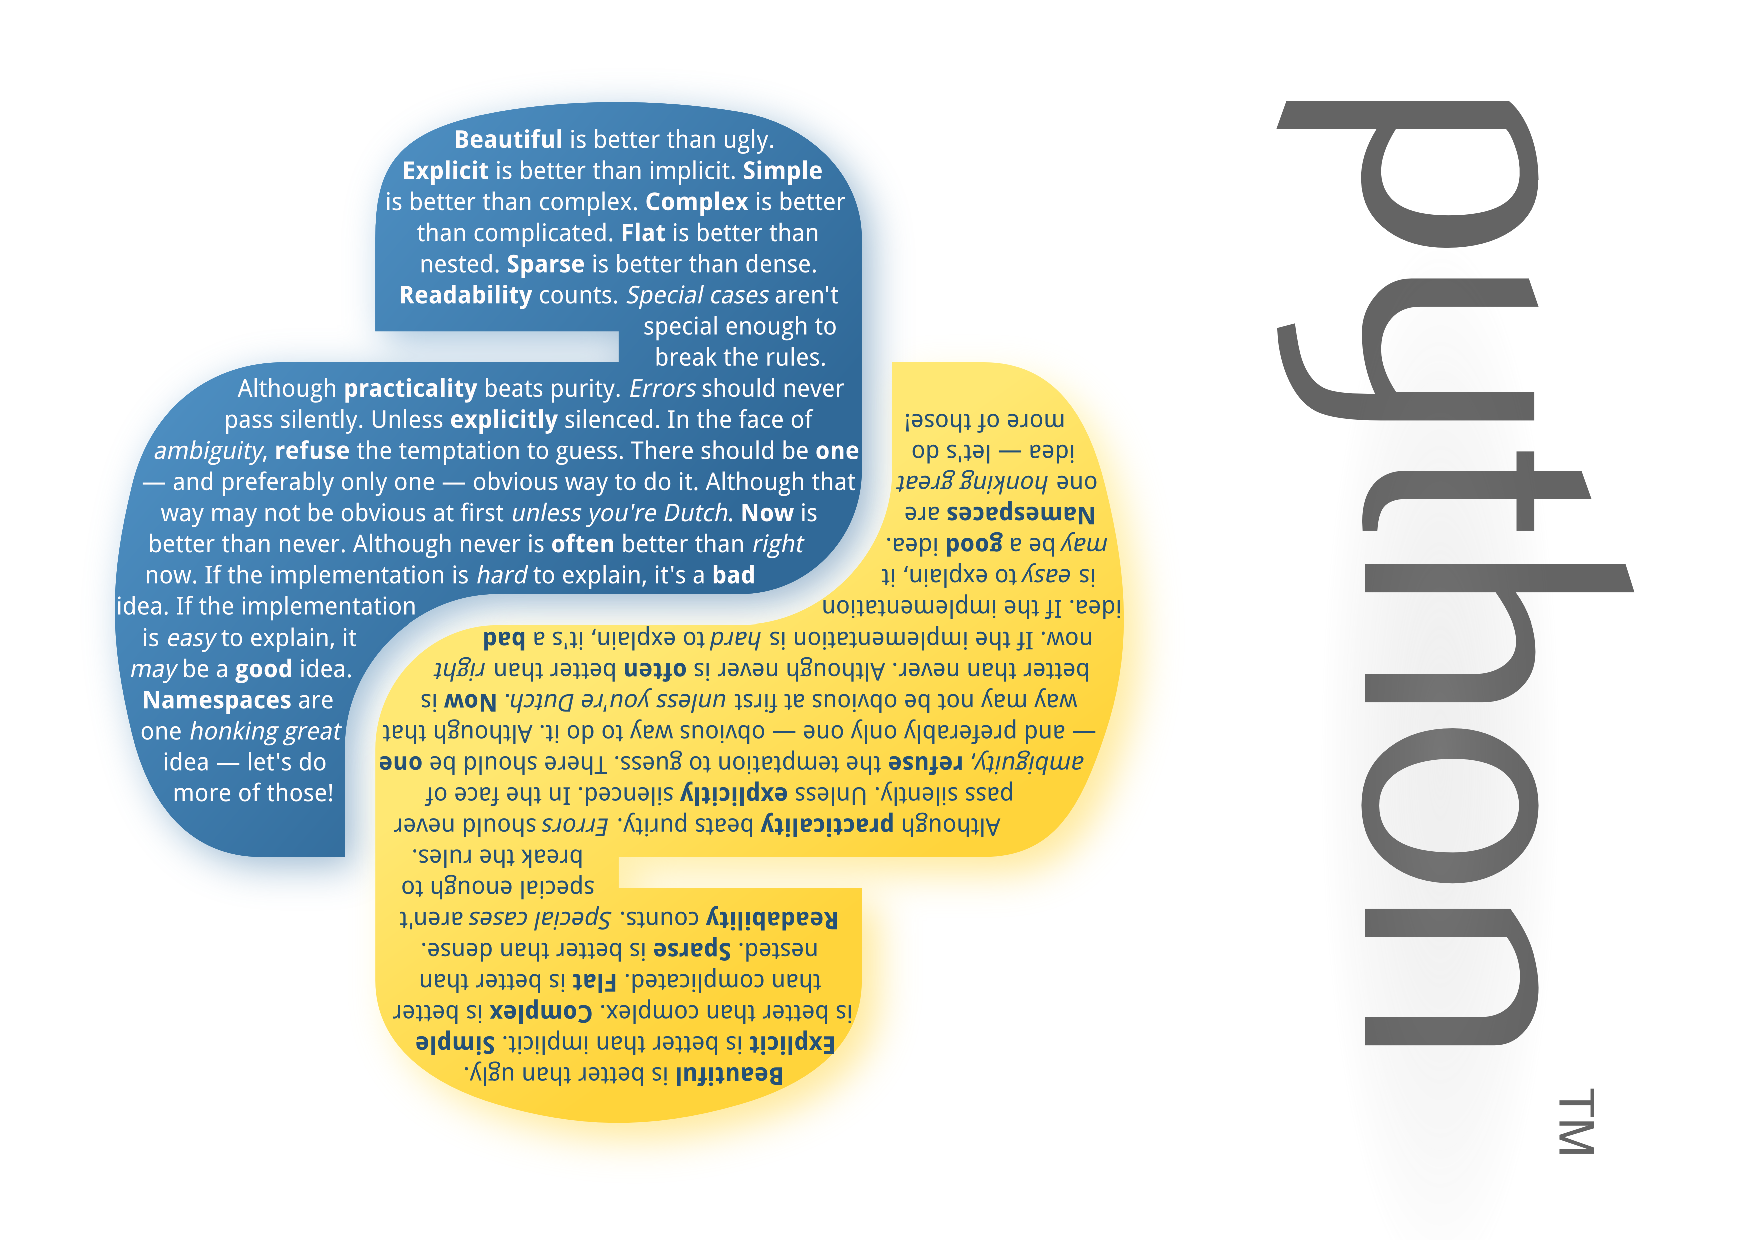
\includegraphics[scale=0.45, clip = true, trim = 0mm  0mm 10cm 0mm]{zen-of-python-poster.pdf}\end{figure}
\end{frame}


\begin{frame}[fragile]
\frametitle{Syntax}
\framesubtitle{Tabs and spaces}
\large
  \begin{columns}[T]
    \begin{column}{.5\textwidth} 
\ \\ 

\ \\ 

\ \\ 
\ \\

\begin{itemize}

% \item $==$  equality \\ \
% \item $!=$ inequality \\ \
%  \item$ >=, >, <=, <$\\ \

\item Syntax is important \ \\
\ \\ 
\item Very important \ \\
\ \\
\item<2-> Comments also
% \item not \\ \

%  \item If not sure, ask Python!


\end{itemize}
     \end{column}
     
         \begin{column}{.5\textwidth} 
\begin{lstlisting}[style=base]
@a = 2@
@b = 8@
@if a == b:@
@2# This is a comment!
  @@print "equal"@
@elif a > b:@
@2# Python ignores me!
  @@print "a is bigger"@
@else:@
@2# But you see me!
  @@print "b is bigger"@
@...@
\end{lstlisting}

    \end{column}
    \end{columns}

%More content goes here
\end{frame}


\begin{frame}[fragile]
\frametitle{Conditional statements}
\framesubtitle{If, then, else}
\large
  \begin{columns}[T]
    \begin{column}{.5\textwidth} 


\begin{itemize}

% \item $==$  equality \\ \
% \item $!=$ inequality \\ \
%  \item$ >=, >, <=, <$\\ \

\item<1-> {If X is the case, then do Y}

\ \\

\ \\

\item<3-> but if A is the case, do B

\ \\
\ \\


\item<3-> but if C is the case, do D

\ \\
\ \\


\item<3-> ...

\ \\

\ \\

\item<2-> otherwise do Z

% \item not \\ \

%  \item If not sure, ask Python!


\end{itemize}
     \end{column}     
         \begin{column}{.5\textwidth} 
\begin{lstlisting}[style=base]
@1a = 2@
@1b = 8@
@1if a == b:@
@1 #a and b the same
@@1 print "equal"@
@3elif a > b:@
@3 #b smaller than a
@@3 print "a is bigger"@
@2else:@
@2 #a smaller than b
@@2 print "b is bigger"@
\end{lstlisting}

    \end{column}
    \end{columns}

%More content goes here
\end{frame}



\begin{frame}[fragile]
\frametitle{For loops}
\framesubtitle{What sorcery is this?}
\large
  \begin{columns}[T]
    \begin{column}{.5\textwidth} 


\begin{itemize}

% \item $==$  equality \\ \
% \item $!=$ inequality \\ \
%  \item$ >=, >, <=, <$\\ \

\item<1-> {Do something}

\ \\

\ \\

\item<2-> {do something}

\ \\
\ \\


\item<3-> {do something}

\ \\
\ \\


\item<4-> {do something}

\ \\

\ \\

\item<5-> {do something}


% \item not \\ \

%  \item If not sure, ask Python!


\end{itemize}
     \end{column}
     
         \begin{column}{.5\textwidth} 
         Text editor:
\begin{lstlisting}[style=base]
@1print 1@
@2print 2@
@3print 3@
@4print 4@
@5print 5@

\end{lstlisting}

Python output:\begin{lstlisting}[style=base]
@61@
@62@
@63@
@64@
@65@


\end{lstlisting}

    \end{column}
    \end{columns}

%More content goes here
\end{frame}





\begin{frame}[fragile]
\frametitle{For loops}
\framesubtitle{What sorcery is this?}
\large
  \begin{columns}[T]
    \begin{column}{.5\textwidth} 


\begin{itemize}

% \item $==$  equality \\ \
% \item $!=$ inequality \\ \
 \item Use a single command! \\ \

\item{Do something five times}


% \item not \\ \

%  \item If not sure, ask Python!


\end{itemize}
     \end{column}
     
         \begin{column}{.5\textwidth} 
         Text editor:
\begin{lstlisting}[style=base]
@for i in range(1,6):@
@  print i@

\end{lstlisting}

\vfill

Python output:
\begin{lstlisting}[style=base]
@21@
@22@
@23@
@24@
@25@


\end{lstlisting}

    \end{column}
    \end{columns}

%More content goes here
\end{frame}




\begin{frame}[fragile]
\frametitle{While loops}
\framesubtitle{More magic!}
\large
%   \begin{columns}[T]
%     \begin{column}{.5\textwidth} 


\begin{itemize}

% \item $==$  equality \\ \
% \item $!=$ inequality \\ \
\item<1->{For loop: for each of the 5 slices of pizza, eat them} \\ \

 \item<2-> What if you don't know how many times you want to do something? \\ \

\item<3->{Do something \emph{until} something else happens} \\ \



\item<4->{While loop: while it's raining, use umbrella}\\ \

\item<5-> While there are slices of pizza, eat them


% \item not \\ \

%  \item If not sure, ask Python!


\end{itemize}
\end{frame}

\begin{frame}[fragile]
\frametitle{While loops}
\framesubtitle{More magic!}

%      \end{column}
     
%          \begin{column}{.5\textwidth} 
         Text editor:
\begin{lstlisting}[style=base]
@1while True:@
    @2n = raw_input("Please enter 'hello':")@
    @3if n == 'hello':@
        @4break@

\end{lstlisting}

\vfill

Python output:
\begin{lstlisting}[style=base]
@5Please enter 'hello':no@
@6Please enter 'hello':never@
@7Please enter 'hello':hi?@
@8Please enter 'hello':hello@
@9>>>@


\end{lstlisting}

%     \end{column}
%     \end{columns}

%More content goes here
\end{frame}


\begin{frame}


\frametitle{Exercises}
\framesubtitle{Do them!}
\huge
\begin{figure}
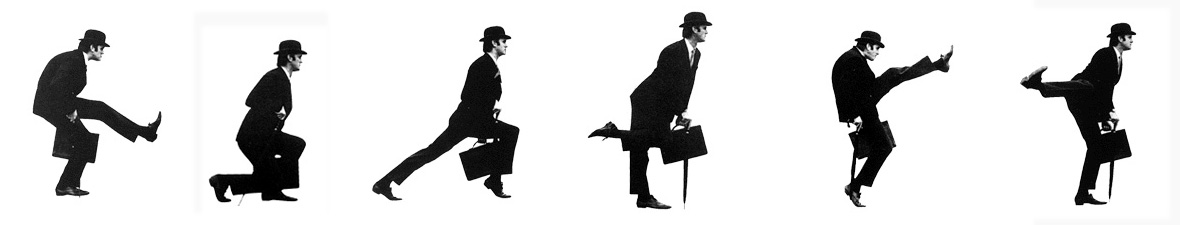
\includegraphics[scale=0.3]{Ministry_of_Silly_walks_2012.jpg}
\end{figure}
 \vfill

\centering Put your hand up if you need help!

\end{frame}



\end{document}
